\chapter{Revisão Sistemática da Literatura}\label{sec:revisaosistematica}
Neste anexo é descrito e discutido uma Revisão Sistemática da Literatura acerca do tema deste trabalho. Na Seção \ref{sec:protocol} é descrito o protocolo seguido para a realização da revisão sistemática. Na Seção \ref{sec:crsl} está o processo de condução da revisão sistemática e quantos artigos veio em cada filtro. Na Seção \ref{sec:results} contém os resultados obtidos, assim como, as respostas para as questões de pesquisa e por fim na Seção \ref{sec:consfi} o resumo e outras discussões sobre esta revisão sistemática da literatura.

\section{Protocolo da Revisão Sistemática da Literatura}\label{sec:protocol}
Este protocolo foi elaborado conforme especificado em: \cite{biolchini2005systematic}, \cite{mafra2006estudos}, e \cite{kitchenham2004procedures}:

\subsection{Objetivo}
O objetivo deste estudo será esquematizado a partir do paradigma GQM (goal, question, and metric) \citep{basili1994experience}:

\begin{table}[]\footnotesize
\centering
\caption{Objetivos da Revisão Sistemática}
\label{my-label}
\begin{tabular}{|
>{\columncolor[HTML]{C0C0C0}}l | M |}
\hline
\textbf{Analisar}              & \begin{tabular}[c]{@{}l@{}}Reconhecimento de emoções por meio da expressão facial em uma imagem\\ estática.\end{tabular} \\ \hline
\textbf{Com o propóstio de}    & Identificar técnicas, métodos, abordagens, arquiteturas, base de dados e aplicações.                                     \\ \hline
\textbf{No que diz respeito a} & Utilização de redes neurais de convolução.                                                                               \\ \hline
\textbf{Do ponto de vista do}  & Pesquisador.                                                                                                             \\ \hline
\textbf{No contexto}           & Acadêmico.                                                                                                               \\ \hline
\end{tabular}
\end{table}


\subsection{Questões de Pesquisa}
\textbf{Questão Principal:} Como reconhecer emoções por meio da expressão facial utilizando redes neurais de convolução em uma imagem estática?
\begin{itemize}
 \item \textbf{Q1}: Quais emoções têm sido reconhecidas por meio da expressão facial utilizando redes neurais de convolução? 
 \item \textbf{Q2}: Quais tipos de pré-processamento tem sido realizado na imagem?
 \item \textbf{Q3}: Quais arquiteturas de redes de convolução têm sido mais utilizadas?
 \item \textbf{Q4}: Quais técnicas, métodos e abordagens têm sido utilizados para tratar problemas na imagem como iluminação, rotação, obstrução e escala?
 \item \textbf{Q5}: Quais bases de dados têm sido utilizadas?
 \item \textbf{Q6}: Quais aplicações podem utilizar o reconhecimento de emoção por expressão facial?
\end{itemize}

\subsection{Biblioteca Digital}
Scopus: \url{http://www.scopus.com/} - Contempla as principais conferências da área (foi verificado por meio de busca manual)

\subsection{Critérios de Inclusão e Exclusão dos Artigos}
\textbf{Critérios de Inclusão:}
\begin{itemize}
 \item \textbf{CI1:} Reconhecimento de emoção por expressão facial usando somente CNN com abordagem que funciona para classificação em imagem;
 \item \textbf{CI2:} Reconhecimento de emoção por expressão facial combinando CNN com várias arquiteturas de redes neurais com abordagem que funciona para classificação em imagem;
 \item \textbf{CI3:} Reconhecimento de emoção por expressão facial combinando CNN com outros métodos de aprendizado de máquina que funciona para classificação em imagem;
 \item \textbf{CI4:} Reconhecimento de emoção por expressão facial combinando CNN com técnicas de pré-processamento que não são originais da arquitetura CNN com abordagem que funciona para classificação em imagem.
 \end{itemize}
 
\textbf{Critérios de Exclusão:}
 \begin{itemize}
  \item \textbf{CE1:} Trabalho somente apresenta teoria ou discussão relacionada ao reconhecimento de emoções;
  \item \textbf{CE2:} Não apresenta reconhecimento de emoção por expressão facial para classificação em imagens;
  \item \textbf{CE3:} Não utiliza redes neurais de convolução;
  \item \textbf{CE4:} Trabalho anterior ao ano de 2013;
  \item \textbf{CE5:} Reconhecimento por vídeo ou \textit{streaming} de imagens;
  \item \textbf{CE6:} Trabalho utiliza durante a metodologia experimental uma base de dados não disponível para a comunidade científica;
  \item \textbf{CE7:} Publicação não disponível;
  \item \textbf{CE8:} Reconhecimento de emoção multimodal.
 \end{itemize}
\textbf{Observação:} O \textit{CE4} foi definido devido o surgimento das (atuais) redes neurais de convolução ter sido a partir de 2013.

\subsection{Formulário de Extração de Informação}
Inicialmente, no primeiro filtro serão analisados e considerados os seguintes itens:
\begin{itemize}
 \item Título;
 \item Resumo;
 \item Palavras-chaves.
\end{itemize}

Posteriormente, no segundo filtro serão extraídas as seguintes informações:
\begin{itemize}
 \item Autores do trabalho;
 \item Fonte: local que o trabalho foi publicado;
 \item Ano de Publicação;
 \item Emoções que foram reconhecidas;
 \item Aplicações para o reconhecimento de emoções por expressão facial;
 \item Arquiteturas de redes neurais de convolução utilizadas;
 \item Metodologia utilizada para o treinamento da rede neural de convolução;
 \item Base de dados utilizadas para treino e validação;
 \item Perspectivas futuras;
 \item Comentários.
\end{itemize}

\subsection{\textit{String} de Busca}\label{sec:stringdebusca} 
As \textit{strings} de busca foram definidas a partir das questões de pesquisa e do padrão PICO (\textit{population}, \textit{intervention}, \textit{comparison}, \textit{outcomes}) (KITCHENHAM e CHARTERS, 2007), conforme a estrutura abaixo:
\begin{itemize}
 \item \textbf{População:} Reconhecimento de emoção por expressão facial;
 \item \textbf{Intervenção:} Por meio de redes neurais de convolução;
 \item \textbf{Comparação:} Não há;
 \item \textbf{Resultados:} Técnicas, métodos, arquiteturas, base de dados, aplicações e abordagens.

 ("emotion recognition"  OR  "emotion detection"  OR  "emotion identification"  OR  "emotion analysis"  OR  "emotion classification"  OR  "affect recognition"  OR  "affect detection"  OR  "affect analysis"  OR  "affect classification"  OR  "facial expression")

 \textbf{AND} 

 ("convolutional neural network"  OR  "CNN"  OR  "long short term memory"  OR  "LSTM"  OR  "recurrent neural network"  OR  "RNN")  

 \textbf{AND}  

 ("technique"  OR  "method"  OR  "architecture"  OR  "database"  OR  "application"  OR  "approach" )
 
 \end{itemize}

Para a montagem da string de busca foi testado cada termo da população com todos os termos da intervenção mais resultado, desta forma, verificando e validando que todos os termos da população realmente contribuem para os artigos retornados. Este mesmo procedimento foi utilizado para verificar e validar os termos do resultado, no entanto foi verificado cada termo do resultado com todos os termos da intervenção e população. 

A presença dos seguintes termos na intervenção: "long short term memory", "LSTM”, "recurrent neural network" e "RNN", podem ser explicados devido à intuição do autor deste protocolo acreditar que a comunidade estava utilizando essas técnicas, que também são redes neurais profundas, combinadas com as redes neurais de convolução para classificação de expressões faciais em imagens.  

\begin{figure}
\centering
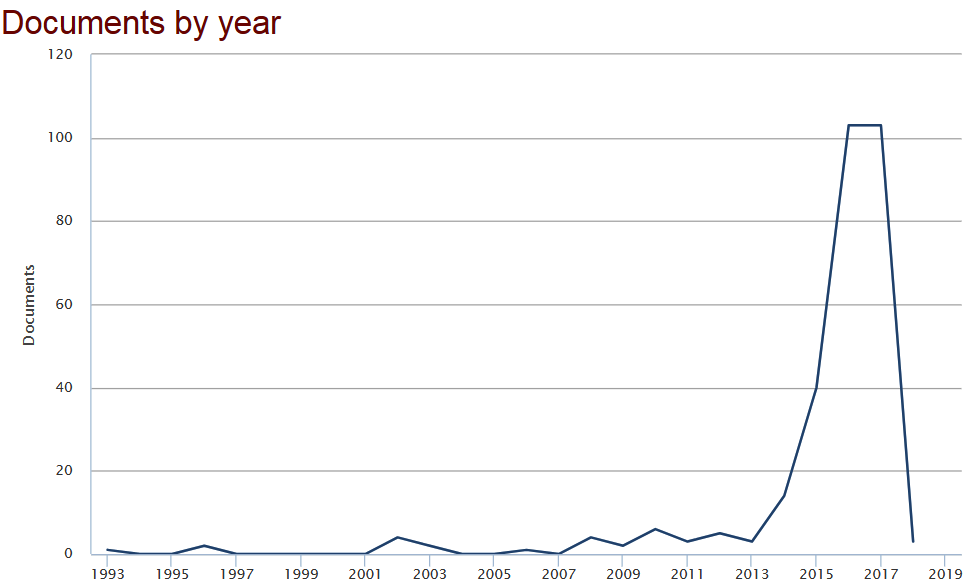
\includegraphics[scale=0.45]{figuras/papersbyyear.png}
\caption{Artigos por ano retornados pela \textit{string} de busca}
\label{fig:papersbyyear}
\end{figure}

\section{Condução da Revisão Sistemática da Literatura}\label{sec:crsl}
\subsection{Primeiro Filtro}
No primeiro filtro foi lido somente o título, resumo e as palavras-chaves do artigo.
A \textit{string} de busca retornou 281 artigos para classificar no primeiro filtro. Foram aceitos 99 (35\%) para o segundo filtro, 3 (1\%) duplicados e 179 (64\%) rejeitados.

Na Seção \ref{sec:stringdebusca}, o autor do protocolo esclarece porque utilizou os seguintes termos na \textit{string} de busca: "long short term memory", "LSTM”, "recurrent neural network" e "RNN", depois do primeiro filtro, realmente comprovou-se que estas técnicas são combinadas com as redes neurais de convolução para classificação de emoção em expressão facial, porém, somente em vídeos ou streaming de imagens. Portanto, os artigos retornados por essas palavras receberam a classificação de rejeitado devido a esta revisão focar em trabalhos com classificação em imagens estática sem streaming. 

\subsection{Segundo Filtro}
Para a realização do segundo filtro foi lido o artigo completo para a extração dos dados e, consequentemente a obtenção dos resultados. No segundo filtro tinham 99 artigos para classificar, onde 34 foram aceitos, 1 duplicados e 64 rejeitados.

\begin{figure}
\centering
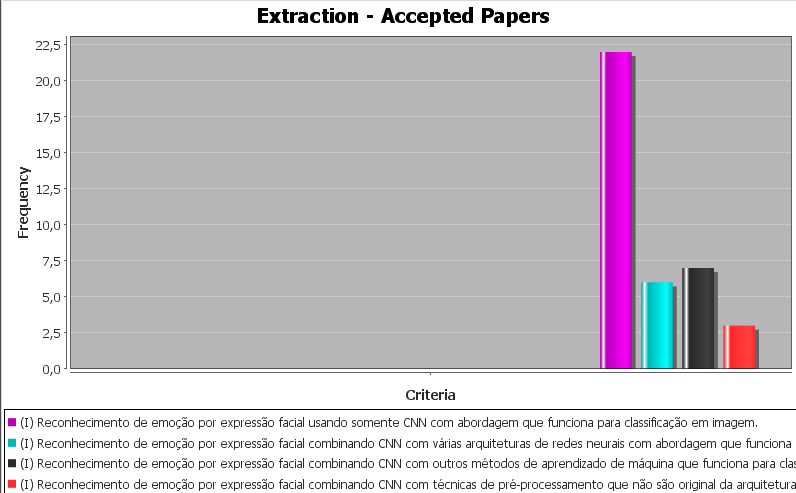
\includegraphics[scale=0.75]{figuras/paperscriteriaaccepted.png}
\caption{Gráfico representando a frequência dos critérios de inclusão para os artigos aceitos do segundo filtro}
\label{fig:papersbyyear}
\end{figure}

\begin{figure}
\centering
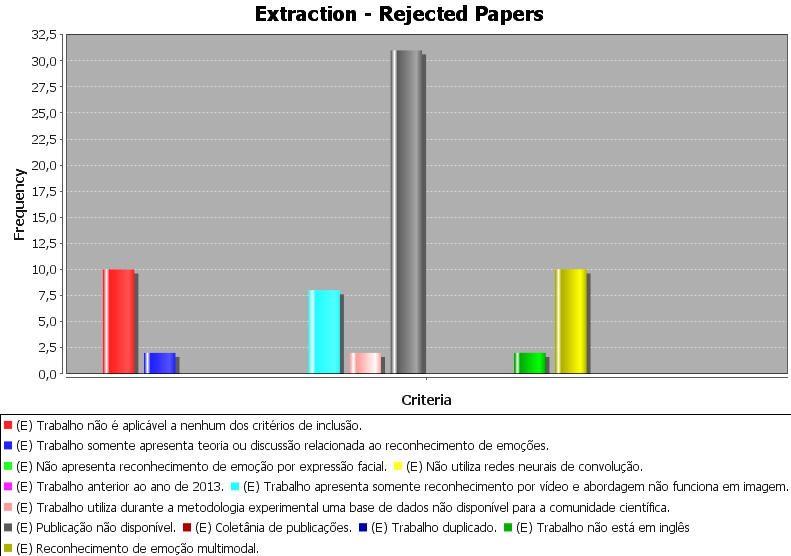
\includegraphics[scale=0.75]{figuras/paperscriteriarejected.png}
\caption{Gráfico representando a frequência dos critérios de exclusão para os artigos rejeitados do segundo filtro}
\label{fig:papersbyyear}
\end{figure}

\section{Resultados}\label{sec:results}
\subsection{Q1: Quais emoções têm sido reconhecidas por meio da expressão facial utilizando redes neurais de convolução?}
As emoções reconhecidas obviamente são as emoções que são representadas e contidas em base de dados, logo são as emoções básicas: neutralidade, felicidade, surpresa, tristeza, raiva, desgosto e medo. Alguns trabalhos como \cite{art8} reconhece também nojo.

\subsection{Q2: Quais tipos de pré-processamento tem sido realizado na imagem?}\label{sec:q2}
Abaixo segue uma lista com o pré-processamento e os trabalhos que fizeram utilização da técnica. 
\begin{itemize}
 \item \textbf{Detector de Face}: Consiste na detecção e recorte da face \citep{art1,art2,art6,art9,art12,art13,art15};
 \item \textbf{Normalização de Brilho (Equalização de histograma)}: Transformada para realce do contraste \citep{art2,art4,art6};
\item \textbf{Normalização Min e Max}: Transformação linear baseada no valor mínimo e máximo da imagem \citep{art4};
\item \textbf{Pontos da Face (pontos geométricos)}: Extração de pontos da face e a distância entre os pontos \citep{art11};
\item \textbf{Escala de Cinza}: Transformação da imagem para escala de cinza \citep{art12};
\item \textbf{Diferença Gaussiana}: Detecta as bordas do objeto, neste caso, evidencia as bordas da face \citep{art6};
\item \textbf{Filtro de Difusão Isotópica}: \citep{art6};
\item \textbf{Normalização DCT}: Transformada discreta do cosseno utilizada em compressão de dados e eventualmente evidenciando informações relevantes da imagem \citep{art6};
\item \textbf{Alinhamento da Face}: Utilização de uma rede neural \textit{autoencoder} para alinhar a face no centro \citep{art4}.
\end{itemize}

\subsection{Q3: Quais arquiteturas de redes neurais de convolução têm sido mais utilizadas?}
A Tabela \ref{arquiteturas} contém as arquiteturas encontradas e os trabalhos que a utilizaram, como podemos verificar a arquitetura AlexNet foi a mais utilizada.

\begin{table}[]\footnotesize
\centering
\begin{tabular}{|c|L|}
\hline
\textbf{Arquitetura} & \textbf{Trabalhos que utilizaram a arquitetura}                                                                                    \\ \hline
AlexNet              & \cite{art1}, \cite{art2}, \cite{art4}, \cite{art7}, \cite{art9}, \cite{art11}, \cite{art13}, \cite{art14}, \cite{art15} \\ \hline
GoogLeNet            & \cite{art10}                                                                                            \\ \hline
VGG                  & \cite{art8}, \cite{art13}                                                                                 \\ \hline
Ensemble             & \cite{art3}, \cite{art5}, \cite{art6}                                                                       \\ \hline
\end{tabular}

\caption{Principais arquiteturas de redes neurais de convolução e os trabalhos que utilizaram}
\label{arquiteturas}

\end{table}

\subsection{Q4: Quais técnicas, métodos e abordagens têm sido utilizados para tratar problemas na imagem como iluminação, rotação, obstrução e escala?}
A principal solução encontrada na literatura foi a ênfase na generalização adequada do aprendizado da rede neural de convolução, isto é, durante a fase de treinamento. Obviamente, as técnicas aplicadas no pré-processamento da imagem (ver Seção \ref{sec:q2}), contribuem para resolver problemas de iluminação por meio da equalização de histograma e de rotação com o alinhamento de face. Entretanto, um achado bastante interessante foi a utilização da técnica de aumento de dados, que consiste durante a fase de treinamento da rede neural de convolução em multiplicar por 10 vezes uma instância (imagem), isto é, gerando 10 novas imagens com pequenos giros da faces, e variações da rotação da pose, escala e iluminação. Acrescendo em 10 vezes o tamanho da base de treinamento, com inserção de variações da imagem resultando em melhor aprendizado da rede.

\subsection{Q5: Quais bases de dados têm sido utilizadas?}
Esta seção tem enfoque nas bases de dados mapeadas para reconhecimento de emoção por expressão facial em uma imagem estática.
Obviamente, é possível encontrar outras base de dados para reconhecimento de emoção que não seja 
por imagem estática, por exemplo, reconhecimento em vídeo, por sensores, em textos e outras.

As bases de dados para reconhecimento de emoção por expressão facial em uma imagem estática tem algo em comum, 
geralmente as amostras de expressões faciais são as mesmas emoções, as chamadas emoções básicas investigadas por \cite{ekman1994}
que são: neutralidade, felicidade, medo, desgosto, raiva, surpresa e tristeza, 
isto significa que são essas as emoções que a comunidade tem reconhecido por expressão facial.
As bases de dados mapeadas podem ser consultadas na Tabela \ref{database}.


\begin{table}\footnotesize
\centering

\begin{tabular}{|c|L|}
\hline
\textbf{Bases de Dados} & \multicolumn{1}{c|}{\textbf{Trabalhos que utilizaram a base para treinamento ou validação}}                                                                                                                  \\ \hline
CK+                    & \cite{art1}, \cite{art2}, \cite{art3}, \cite{art6}, \cite{art7}, \cite{art9}, \cite{art11}, \cite{art12}, \cite{art14}, \cite{art15} \\ \hline
JAFFE                  & \cite{art1}, \cite{art2}, \cite{art3}, \cite{art6}, \cite{art12}                                                                               \\ \hline
FER                    & \cite{art3}, \cite{art4}, \cite{art5}, \cite{art6}, \cite{art7}, \cite{art10}, \cite{art13}, \cite{art14}                                \\ \hline
FER+                   & \cite{art8}                                                                                                                                            \\ \hline
SFEW2.0                & \cite{art6}, \cite{art10}                                                                                                                            \\ \hline
KDEF                   & \cite{art6}                                                                                                                                            \\ \hline
MMI                    & \cite{art11}                                                                                                                                           \\ \hline
CIFE                   & \cite{art15}                                                                                                                                           \\ \hline
EmotiW2015             & \cite{art3}, \cite{art13}                                                                                                                            \\ \hline
\end{tabular}

\caption{Bases de Dados}

\label{table:database}
\end{table}



\subsection{Q6: Quais aplicações podem utilizar o reconhecimento de emoção por expressão facial?}
Há diversas aplicações para o reconhecimento de emoção no mundo real, foi percebido que os pesquisadores de reconhecimento de emoção por expressão facial utilizando rede neural de convolução, ultimamente concentraram seus esforços mais no desenvolvimento de reconhecedores de emoção do que a aplicação em cenários reais, mesmo assim, está aberto para trabalhos futuros inúmeras aplicações desses reconhecedores em diversas áreas, tendo destaque principalmente para: 

\begin{itemize}
\item \textbf{Interação humano computador}: no qual pode ser possível projetar interfaces que se adaptam ao estado emocional do usuário \citep{art1, art3, art5,art8};
\item \textbf{Psiquiatria e cuidados médicos}: 
no qual o reconhecedor de emoção deve monitorar constantemente o paciente ou usuário
fornecendo dados emocionais que podem contribuir para diagnósticos \citep{art1, art3, art12};
\item \textbf{Deficiente visual}: pois pessoas com alto grau de deficiência visual, tem dificuldades na
interação entre pessoas para identificar qual a emoção que as pessoas em volta estão emitindo \citep{art15},;
\item \textbf{Interação humano robô}: fazendo com que robôs estejam habilitados
a interagir com humanos podendo adaptar-se a emoção dos humanos em volta, 
ou até mesmo emitir emoção se aproximando de um humanoide \citep{art6, art14};
\item \textbf{Personagens virtuais e animação}: 
habilitando avatares a copiar expressão humana que podem ser útil para gravações de filmes de animação,
também pode ser usado em aplicações de animação como o popular aplicativo para \textit{smartphone} o \textit{Snapchat},
que identifica a expressão facial do usuário e retorna alguma animação sobrepondo a expressão anteriormente detectada do usuário \citep{art9, art11}.
\end{itemize}

\subsection{Questão Principal: Como reconhecer emoções por meio da expressão facial utilizando redes neurais de convolução em uma imagem estática?}
Diante das fichas de extração, foi percebido que a comunidade explorou diversas estratégias para processar imagens de expressão facial e reconhecer emoção. Algumas abordagens se destacam como: a técnica para aumentar os dados de treinamento e teste, utilizando a técnica flip fazendo até 10 pequenas rotações na imagem, para a CNN aprender a generalizar melhor sendo treinada e testada com uma base de dados maior. A técnica de normalização de brilho (equalização) no pré-processamento, no qual todos os trabalhos que utilizaram esta técnica aumentaram a acurácia do reconhecimento. Também merece destaque o trabalho de \cite{kim2016fusing} em que na sua abordagem, a rede de convolução recebe duas expressões faciais de entrada: a saída de um autoencoder que alinha a face e a imagem original sem alinhamento da face. Esta abordagem melhorou bastante o reconhecimento.

Com relação à arquitetura da rede neural de convolução, quem utilizou um SVM como classificador ao invés de um tradicional softmax obteve maior acurácia. Teve trabalhos que utilizou uma rede com camadas inceptions, hipergrafo, ensembles e concatenação de redes, e todas essas abordagens superaram uma CNN simples. Neste caso, falta um trabalho que possa dizer experimentalmente qual dessas arquiteturas é a melhor. 

Percebemos que existem várias bases de dados disponíveis para a comunidade. As bases de dados que foram mais exploradas foram a CK+, FER2013 e a JAFFE. A base CK+ é composta por expressões faciais capturadas em laboratório, por isso, tem altas taxas de reconhecimento, pois, sua dificuldade para o reconhecimento diminui. Já a base FER2013 foi capturada na “natureza”, por isso sua taxa de reconhecimento é mais baixa sendo uma base bastante complexa para classificação.

Notoriamente os trabalhos utilizam o algoritmo Viola Jones para detecção de face pelo programa OpenCV e fazem o recorte da face excluindo o background. Desta forma, elimina o trabalho da rede em aprender a separar o que é background e o que é face, diminuindo a complexidade da classificação.

Portanto, para reconhecer emoção em uma imagem estática, é necessário o treinamento de uma rede de convolução com um classificador na última camada, com a maior quantidade de dados possível, realizando o recorte da face e utilizar técnicas de normalização na imagem, ocasionando um aumento da taxa de reconhecimento. 

\section{Resumo}\label{sec:consfi}
Neste anexo apresentou uma revisão sistemática da literatura que investigou o estado-da-arte sobre o reconhecimento de emoção por expressão facial por meio de redes neurais de convolução. Verificamos que o tema está bem quente na comunidade, pois, antes de 2013 a String de busca retornou 33 artigos, e em 2013 (3 artigos), 2014 (14 artigos), 2015 (40 artigos), 2016 (103 artigos), 2017 (103 artigos) e 2018 (3 artigos), isso demonstra o crescimento exponencial da área.

Foram mapeadas as principais técnicas de pré-processamento, arquitetura de rede neural de convolução, base de dados, metodologias de treinamento e aplicações do reconhecimento de emoção. A impressão que fica é que a comunidade ainda não está utilizando esses classificadores no mundo real, e o amadurecimento rápido da área depois do surgimento do aprendizado profundo, nos levar acreditar que esses sistemas já estão prontos para ser posto em prática apoiando outras aplicações de interação humano computador, interação humano robô, educação, segurança, computação afetiva e etc.
